%% ****** Start of file apstemplate.tex ****** %
%%
%%
%%   This file is part of the APS files in the REVTeX 4.2 distribution.
%%   Version 4.2a of REVTeX, January, 2015
%%
%%
%%   Copyright (c) 2015 The American Physical Society.
%%
%%   See the REVTeX 4 README file for restrictions and more information.
%%
%
% This is a template for producing manuscripts for use with REVTEX 4.2
% Copy this file to another name and then work on that file.
% That way, you always have this original template file to use.
%
% Group addresses by affiliation; use superscriptaddress for long
% author lists, or if there are many overlapping affiliations.
% For Phys. Rev. appearance, change preprint to twocolumn.
% Choose pra, prb, prc, prd, pre, prl, prstab, prstper, or rmp for journal
%  Add 'draft' option to mark overfull boxes with black boxes
%  Add 'showkeys' option to make keywords appear
%\documentclass[aps,prl,preprint,groupedaddress]{revtex4-2}
%\documentclass[aps,prl,preprint,superscriptaddress]{revtex4-2}
%\documentclass[aps,prl,reprint,groupedaddress]{revtex4-2}
\documentclass[aps,prb,reprint,superscriptaddress]{revtex4-2}

\usepackage{blindtext}
\usepackage{mhchem}
\usepackage{hyperref}
\usepackage{bm}
\usepackage{siunitx}
\usepackage{mathrsfs}
\usepackage{csquotes}

\graphicspath{{source/}}

% You should use BibTeX and apsrev.bst for references
% Choosing a journal automatically selects the correct APS
% BibTeX style file (bst file), so only uncomment the line
% below if necessary.
%\bibliographystyle{apsrev4-2}

\begin{document}

% Use the \preprint command to place your local institutional report
% number in the upper righthand corner of the title page in preprint mode.
% Multiple \preprint commands are allowed.
% Use the 'preprintnumbers' class option to override journal defaults
% to display numbers if necessary
%\preprint{}

%Title of paper
\title{Self-organized criticality and clumpy sandpiles}

% repeat the \author .. \affiliation  etc. as needed
% \email, \thanks, \homepage, \altaffiliation all apply to the current
% author. Explanatory text should go in the []'s, actual e-mail
% address or url should go in the {}'s for \email and \homepage.
% Please use the appropriate macro foreach each type of information

% \affiliation command applies to all authors since the last
% \affiliation command. The \affiliation command should follow the
% other information
% \affiliation can be followed by \email, \homepage, \thanks as well.
\author{Bryan T. Fichera}
\affiliation{Department of Physics, Massachusetts Institute of Technology, Cambridge, Massachusetts 02139, USA}
\email[]{bfichera@mit.edu}
%\homepage[]{Your web page}
%\thanks{}
%\altaffiliation{}

%Collaboration name if desired (requires use of superscriptaddress
%option in \documentclass). \noaffiliation is required (may also be
%used with the \author command).
%\collaboration can be followed by \email, \homepage, \thanks as well.
%\collaboration{}
%\noaffiliation

\date{\today}

\begin{abstract}
% insert abstract here
In this term paper, I discuss a type of dynamical critical phenomena known as self-organized criticality, which in contrast to the critical phases presented in class does not require any external tuning parameters. I give an introduction to the simplest model exhibiting self-organized criticality, the abelian sandpile model, and discuss some of the associated phenomenology. Examples are given of self-organized criticality in nature, and key ingredients for self-organized criticality are identified. Lastly, a brief review of the literature concerning the effect of defects on self-organized criticality is provided, as well as first-pass numerical simulations on a model of my own construction which I call the ``clumpy sandpile'' model, in which defects are inherent to the particles of the model rather than static features of the environment.
\end{abstract}

% insert suggested keywords - APS authors don't need to do this
%\keywords{}

%\maketitle must follow title, authors, abstract, and keywords
\maketitle

\section{Introduction}

A key aspect of the types of phase transitions that we have covered in 8.334 was the concept of a critical point. A system at its critical point is characterized by total scale invariance, in the sense that its relevant correlation lengths are divergent and its correlation functions decay like power laws with separation. The concept of scale invariance was used to illuminate the notion of universality, i.e. the (experimental) observation that disparate systems with tangible microscopic differences behaved the same way (in the sense of macroscopic observables scaling equivalently with temperature or other parameters) near the critical point. The critical point itself was found to be a single point or line in the space of the tuning parameters, but an entire volume (with co-dimension equal to the number of tuning parameters) in the space of all parameters (both microscopic and macroscopic) relevant to the system.

Therefore, in these systems to reach a critical point it was necessary to drive the system by some combination of external parameters like temperature, pressure, or magnetic field. In addition, the critical point was always unstable to small fluctuations in the tuning parameters, so that a state of persistent criticality was not practically possible. While this is certainly characteristic of the majority of physical systems in the everyday world, there are in fact a variety of other systems for which criticality -- in the sense of divergent correlation lengths, power law decay of correlation functions, and inherent scale invariance -- is rather an emergent property, which arises naturally without any fine-tuning of experimental parameters\cite{jensen, otherbook}. This phenomenon has been called ``self-organized criticality'' (SOC), and is thought to underpin the physics of a number of natural critical phenomena such as earthquakes, forest fires, and droplet formation, which display critical behavior in the absence of tuning parameters.

In this term paper, I discuss a simple lattice model exhibiting SOC known as the abelian sandpile model (ASM). First I give a brief overview of the ASM, including a discussion of the critical phenomenology. Then, I discuss some physical realizations of the model, and review the literature regarding defects in the ASM. Finally, I simulate a variant of the ASM in which defects are attached to individual particles rather than features of the environment, and discuss the question of whether SOC or universality exists in the model.

\section{The abelian sandpile model}

\subsection{Definition\label{sec:rules}}

The ASM was discovered in 1987 by Bak, Tang, and Wiesenfeld as the first example of a dynamical system exhibiting self-organized criticality~\cite{bak_self-organized_1987}. At a schematic level, the model consists of a $d$-dimensional lattice whose sites are described as containing an integer number of grains of sand. At any given site, if the number of grains is greater than some threshold value then the site ``topples,'' scattering its sand to its nearest neighbors. A single step of the evolution of the system consists of randomly adding one grain of sand to the lattice, and then relaxing the system by some defined toppling rules. After the system is stable with respect to those toppling rules, then another grain of sand is added to a random site and the evolution continues. In this respect, the drive frequency of the ASM is said to be much smaller than the relaxation rate.

Mathematically, the ASM can be defined as follows~\cite{majumdar_equivalence_1992, bak_self-organized_1987, dhar_self-organized_1990}. Let $z_i$ be the number of grains at site $i$, $1 \leq i \leq N$ on a given lattice with $N$ sites, and let each site be assigned a threshold value $\Delta_{ii}$. Then evolve the system according to the following rules~\cite{dhar_self-organized_1990}:

\begin{enumerate}
\item[(i)] Choose an integer $i$ randomly from $[1, N]$. Take $z_i \rightarrow z_i+1$.
\item[(ii)] For each $j$ such that $z_j \geq \Delta_{jj}$, perform a topple at site $j$ according to the toppling rule:
\begin{enumerate}
\item[(i.a)] For each integer $k \in [1, N]$, take $z_k \rightarrow z_k - \Delta_{jk}$.
\end{enumerate}
\item[(iii)] Repeat (ii) until there are no integers $j$, $1 \leq j \leq N$ such that $z_j \geq \Delta_{jj}$.
\item[(iv)] Repeat from (i).
\end{enumerate}

An additional requirement of the ASM is that the system lose some amount of sand to dissipation, or else continual evolution of the system will simply result in a state with high density and infinite toppling time~\cite{jensen}. Note that with this condition, $\sum_j\Delta_{ij} \geq 0$ for all $i$~\cite{majumdar_equivalence_1992}. Dissipation is typically introduced using so-called open boundary conditions, where the sandpile is said to exist on a table such that grains of sand can topple over the edge, where they disappear.

An illustration of a simple 2-dimensional ASM is given in Fig.~\ref{fig:rules}. It can be shown~\cite{dhar_self-organized_1990} that the toppling rules described above give rise to relaxation rules that are abelian, in the sense that a state where multiple sites are above the threshold will always relax to the same final state, regardless of the order in which the critical sites are toppled.

\begin{figure}
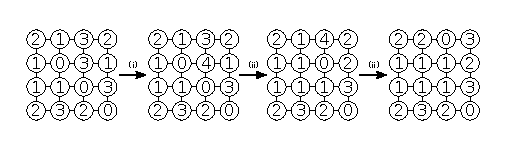
\includegraphics{rules}
\caption{\label{fig:rules} An illustration of the ASM toppling rules (section~\ref{sec:rules}) in the simple case of a $4 \times 4$ square lattice with open boundary conditions, with $\Delta_{ij} = -1$ if sites $i$ and $j$ are nearest neighbors, $\Delta_{ij} = 4$ if $i = j$, and $\Delta_{ij} = 0$ otherwise.}
\end{figure}

\subsection{Phenomenology\label{sec:phenomenology}}

In the ASM, there are in general three quantities which are used to study the dynamical properties~\cite{jensen, otherbook}. First, define for a given avalanche

\begin{enumerate}
\item[(i)] $n$, the number of topples involved in the avalanche before the system relaxes to a stable state,
\item[(ii)] $t$, the number of time steps required for the relaxation process (the ``lifetime'' of the avalanche),
\item[(iii)] $l$, the linear size of an avalanche (which reaches sites at positions $\{\bm{r}_i$\}), defined by
\[
l = \dfrac{1}{|A|}\sum_i|\bm{r}_i-\bm{R}_{cm}|,
\]
where
\[
\bm{R}_{cm} = \dfrac{1}{|A|}\sum_i\bm{r}_i
\]
and the avalanche reaches $A$ distinct points.
\end{enumerate}

Of course the above quantities are not independent, so to discuss the statistical nature of the system it is necessary to study the joint probability distribution for avalanches $P(n, t, l)$. However, this is computationally quite difficult so that researchers mostly study the unconditional probability distributions $P(n)$, $P(t)$, and $P(l)$, where $P(x)$ is the probability that a given avalanche has property $x$, irrespective of the other two quantities. The ASM is said to exhibit self-organized criticality because the probabilities $P(n)$, $P(t)$, and $P(l)$ are power law distributed in their arguments~\cite{jensen}.

To show that the ASM exhibits self-organized criticality, I performed simulations of an ASM on a 2-dimensional $20 \times 20$ square lattice with open boundary conditions, nearest-neighbor toppling rules like those in Fig.~\ref{fig:rules}, and $\Delta_{ii} = 4$ for all $i$. Fig.~\ref{fig:density} shows the approach to criticality in the density $\rho$ of sand grains in the lattice. Histograms of avalanche sizes and lifetimes in the simulation are plotted in Fig.~\ref{fig:avalanches}(a) and (b), respectively.

\begin{figure}
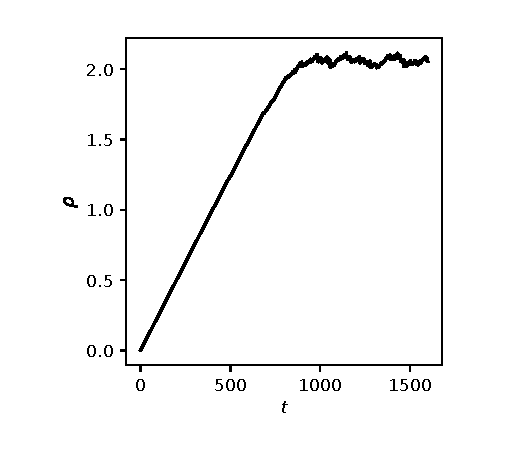
\includegraphics{density}
\caption{\label{fig:density} Approach to criticality of the 2-dimensional ASM on a square lattice, measured by the density of sand grains $\rho$ as a function of time $t$. The stationary value of $\rho \approx \rho_c = 2.12$ is typical for the ASM on a 2-dimensional square grid~\cite{jensen}.}
\end{figure}

\begin{figure}
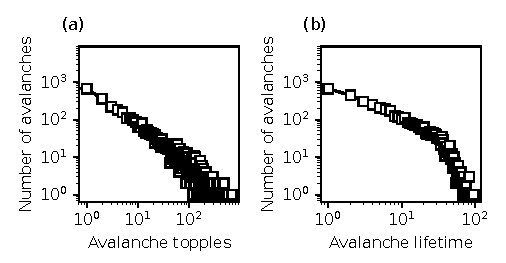
\includegraphics{avalanches}
\caption{\label{fig:avalanches}Histogram of avalanche sizes (in number of topples), (a) and avalanche lifetimes (b) after $10000$ drive periods on a 2-dimensional $20 \times 20$ square ASM with open boundary conditions, nearest-neighbor toppling rules like Fig.~\ref{fig:rules}, and $\Delta_{ii} = 4$ for all $i$. The histograms show power law behavior over 1-2 decades. Deviations from power law behavior are likely due to finite-size effects~\cite{jensen}.}
\end{figure}

\section{SOC in nature}

A number of systems which are encountered in physics exibit behavior which is similar to that of the ASM. As a matter of fact, there is reason to suspect that the ASM can actually provide a good description of those systems, if not quantitatively than at least qualitatively. This is because the aspects of the ASM which are thought to be essential for SOC, namely that the system exhibit threshold behavior and be driven at a low frequency compared to the relaxation rate, are readily apparent in these systems. A classic example is the Earth's crust, where, as in the ASM, long periods of structural stability are interrupted by violent releases of energy known as earthquakes. That the speed of the Earth's crust in the stationary state -- a few centimeters per year -- is so much slower than during an earthquake constitutes the condition that the drive period be much longer than the relaxation time. Moreover, the system naturally involves threshold behavior, as tectonic plates slip past one another only when the associated stress passes the threshold set by the effective coefficient of static friction. And indeed, measurable quantities in the system like the probability $P(E)$ that an earthquake dissipate energy $E$ have been shown to be power law-distributed and scale invariant~\cite{jensen}.

While the Earth's crust is certainly the case in which the application of SOC has been the most successful, many other systems also exhibit SOC behavior. For example, the coalescence of droplets of water into ``rivers'' on a glass surface has been shown to exhibit power law behavior like in the ASM~\cite{jensen, plourde_water_1993}. In type II superconductors, magnetic flux vortices can accumulate on material defects to some threshold concentration until their mutual repulsion forces them away, a phenomenon which has been shown to exhibit power law-distributed event sizes and frequencies~\cite{field_superconducting_1995}. It has even been posited that the interruption of long periods of slow biological evolution by rapid explosions of species diversity could be an example of SOC~\cite{raup_biological_1986}. While SOC may not be able to account for all of the quantitative and qualitative features of these systems, it at least provides as qualitative paradigm for interpreting the existence of critical behavior in the absence of tuning parameters.

\section{Defects in sandpile models}

While many variants of the ASM have been studied by researchers since the model's discovery in 1987, in the course of my research I have become particularly interested in the effects of defects to the model. There are many interesting questions to be asked when considering the effect of defects in the ASM, but one in particular which has caught some attention is the question of whether a given system still displays SOC upon the introduction of a finite concentration of defects. The question has been explored by introducing defects of various kinds to the model and investigating the distribution functions described in section~\ref{sec:phenomenology}.

By far the most common type of defect which has been studied in the ASM is a dissipative defect. In 1992, Tadic \textit{et al.} studied the ASM with a random distribution of holes through which sand can leave the system~\cite{tadic_scaling_1992}. They find with numerical analysis that SOC in the modified ASM is destroyed at long time scales and length scales for any finite concentration of holes (see Fig.~\ref{fig:defects}). This conclusion was later supported by mean field and renormalization group analysis~\cite{ghaffari_nonconservative_1997}. More general nonconservative (in the sense of particle number, excluding boundaries) ASMs were also found to move away from criticality for an arbitrarily small amount of dissipation~\cite{tsuchiya_proof_2000}. These studies have shown that the vanishing of the drive frequency and the presence of threshold toppling rules are necessary, but not sufficient conditions for SOC in the ASM.

\begin{figure}
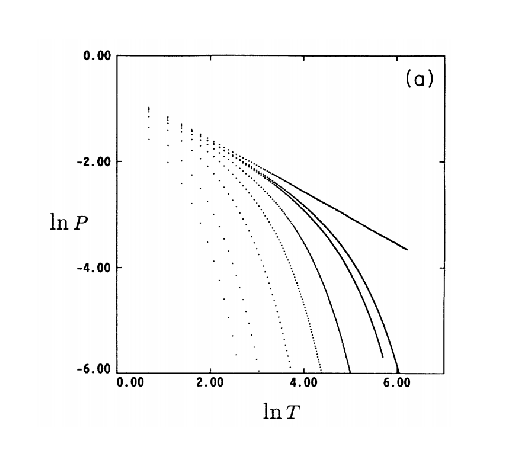
\includegraphics{defects}
\caption{\label{fig:defects} The probability distribution, $P$ against the duration of avanlanches, $T$ for concentrations of defects (from top to bottom) $0.0$, $0.0075$, $0.025$, $0.05$, $0.1$, $0.2$, $0.295$. The loss of criticality is evidenced by the lack of power law behavior in $P$ for nonzero defect concentration. After Ref.~\onlinecite{tadic_scaling_1992}}
\end{figure}

\section{Clumpy sandpiles}

In contrast, we may also imagine a model in which the toppling rules are conservative, but the distribution of sand ``masses'' differs from that of the simple ASM. In this way, the ``defects'' in the model are not defects of the lattice, but rather mobile defects in the form of sand grains which carry more or less weight than in the original model. One can ask, as a function of some reasonably-defined deviation from a sharp mass distribution, does the system exhibit SOC and does it belong to the same universality class as the original model?

To answer this question, I performed numerical simulations on a variant of the ASM in which at each driving step a grain of sand is randomly added to the lattice, where the mass of the grain of sand is 1 with probability $p$ and 2 with probability $1-p$ (one can think of the heavier grain as a ``clump''). A site $i$ is stable when its total mass $m_i$ satisfies $m_i < 4$. If $m_i \geq 4$, the site topples, and a number of grains are distributed randomly to nearest neighbor sites such that the total mass distributed is 4, and that no site receives two grains of sand in the same topple (for concreteness, in a given topple event we distribute heavy grains first, and then distribute the lighter grains). The system is equivalent to the ASM for $p = 1$. Physically, one could imagine this model as pertaining to the dynamics of magnetic flux vortices in a dirty superconductor where the vortices are allowed to carry more than one flux quantum.

I simulated the above ``clumpy sandpile'' model on a $50 \times 50$ 2-dimensional square lattice with open boundary conditions, and studied the behavior of the model as a function of $p$. First, for each $p$ I verified that a stationary (if not necessarily critical) state does exist, by monitoring the density with time as in Fig.~\ref{fig:density}. Then, I ran $10000$ driving periods of the evolution, and recorded for each avalanche the number of topples $s$ and the relaxation time $t$. The question of whether the system exhibits SOC can be investigated by studying the distribution functions described in section~\ref{sec:phenomenology}.

\begin{figure}
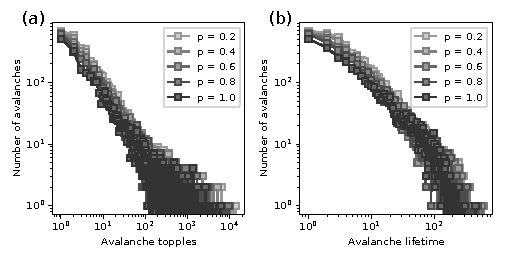
\includegraphics{avalanches_p}
\caption{\label{fig:avalanches_p} Distribution functions in the clumpy sandpile model for (a) avalanche size (in number of topples) and (b) avalanche lifetime as a function of $p$.}
\end{figure}

The results of the simulations are shown in Fig.~\ref{fig:avalanches_p}. It appears that the relevant distribution functions still exhibit power law behavior in the ``clumpy'' sandpile model, at least for a reasonable range given the size of the lattice and the length of the simulation. However, it is impossible to say for certain whether the system is truly critical without a formal proof, or at the very least better numerics (the simulations were sorely limited by lack of computational power).

\begin{figure}
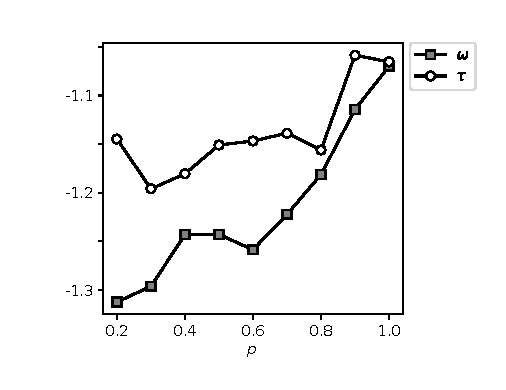
\includegraphics{exps}
\caption{\label{fig:exps} Critical exponents of the clumpy sandpile model extracted from Fig.~\ref{fig:avalanches_p}, as a function of $p$.}
\end{figure}

Using the distribution functions in Fig.~\ref{fig:avalanches_p}, it is possible to calculate the critical exponents $\tau$ and $\omega$ (defined so that $P(t) \sim t^\omega$ and $P(s) \sim s^\tau$ for avalanches of $s$ topples and lifetimes of $t$) as a function of $p$. The results are plotted in Fig.~\ref{fig:exps}. I find evidence that the exponent $\tau$ may change with $p$, whereas the evidence is less obvious for the exponent $\omega$. This suggests that $p\neq 1$ may be driving the model away from universality. However, it should again be cautioned that this question could be investigated with much better accuracy given greater computational power.

\section{Conclusion}

In this term paper, I have discussed SOC in contrast to the models of criticality discussed in class. I have described the simplest model exhibiting SOC, the ASM, and discussed the model phenomenologically in terms of critical exponents and distribution functions. Physical systems were identified which display SOC, and key ingredients for SOC, including threshold dynamics and vanishing drive frequency, were highlighted. Lastly, I discussed the literature surrounding defects in the ASM, and presented some rudimentary simulations of a model where defects are native to the grains themselves rather than features of the environment. It was found that the model appeared to exhibit some features of SOC, including power law scaling of distribution functions, but that the critical exponents changed with the ``clumpiness'' of the model. Greater computational capacity will be necessary to investigate the clumpy sandpile model, and analytical investigations should be carried out to discern the nature of the associated stationary phase.

All source code can be found at \url{https://github.com/bfichera/asm}. I gratefully acknowledge Mehran Kardar for his mentorship in 8.334, as well as Abe Levitan and Camilla Schneier for helpful discussions. 
\bibliography{asm}

\end{document}
